\subsection{Calibration}

First we have to calibrate the system. We only measure the number of entries in different channels, but we know at which energies the spectrum of ${}^{22}\mathrm{Na}$, $^{60}\mathrm{Co}$ and $^{137}\mathrm{Cs}$ have peaks due to radiation. With these values we can make a linear regression and map the channels onto energies. \\
Fig.2.1 shows the entries in each channel for ${}^{22}\mathrm{Na}$ as an example. We fitted the peaks with gaussian functions to get better estimated values. \\
In Fig.2.2 you can see the channels of each peak and the corresponding energies. Fig.2.3 finally shows the linear regression with the following parameters:
$$\mathrm{y-intercept} = (-3.02810 \pm 1.48205) \cdot 10^{2} \ keV$$
$$\mathrm{slope} =  (3.64232 \pm 0.513385) \ keV$$

\begin{figure}[h]
\centering
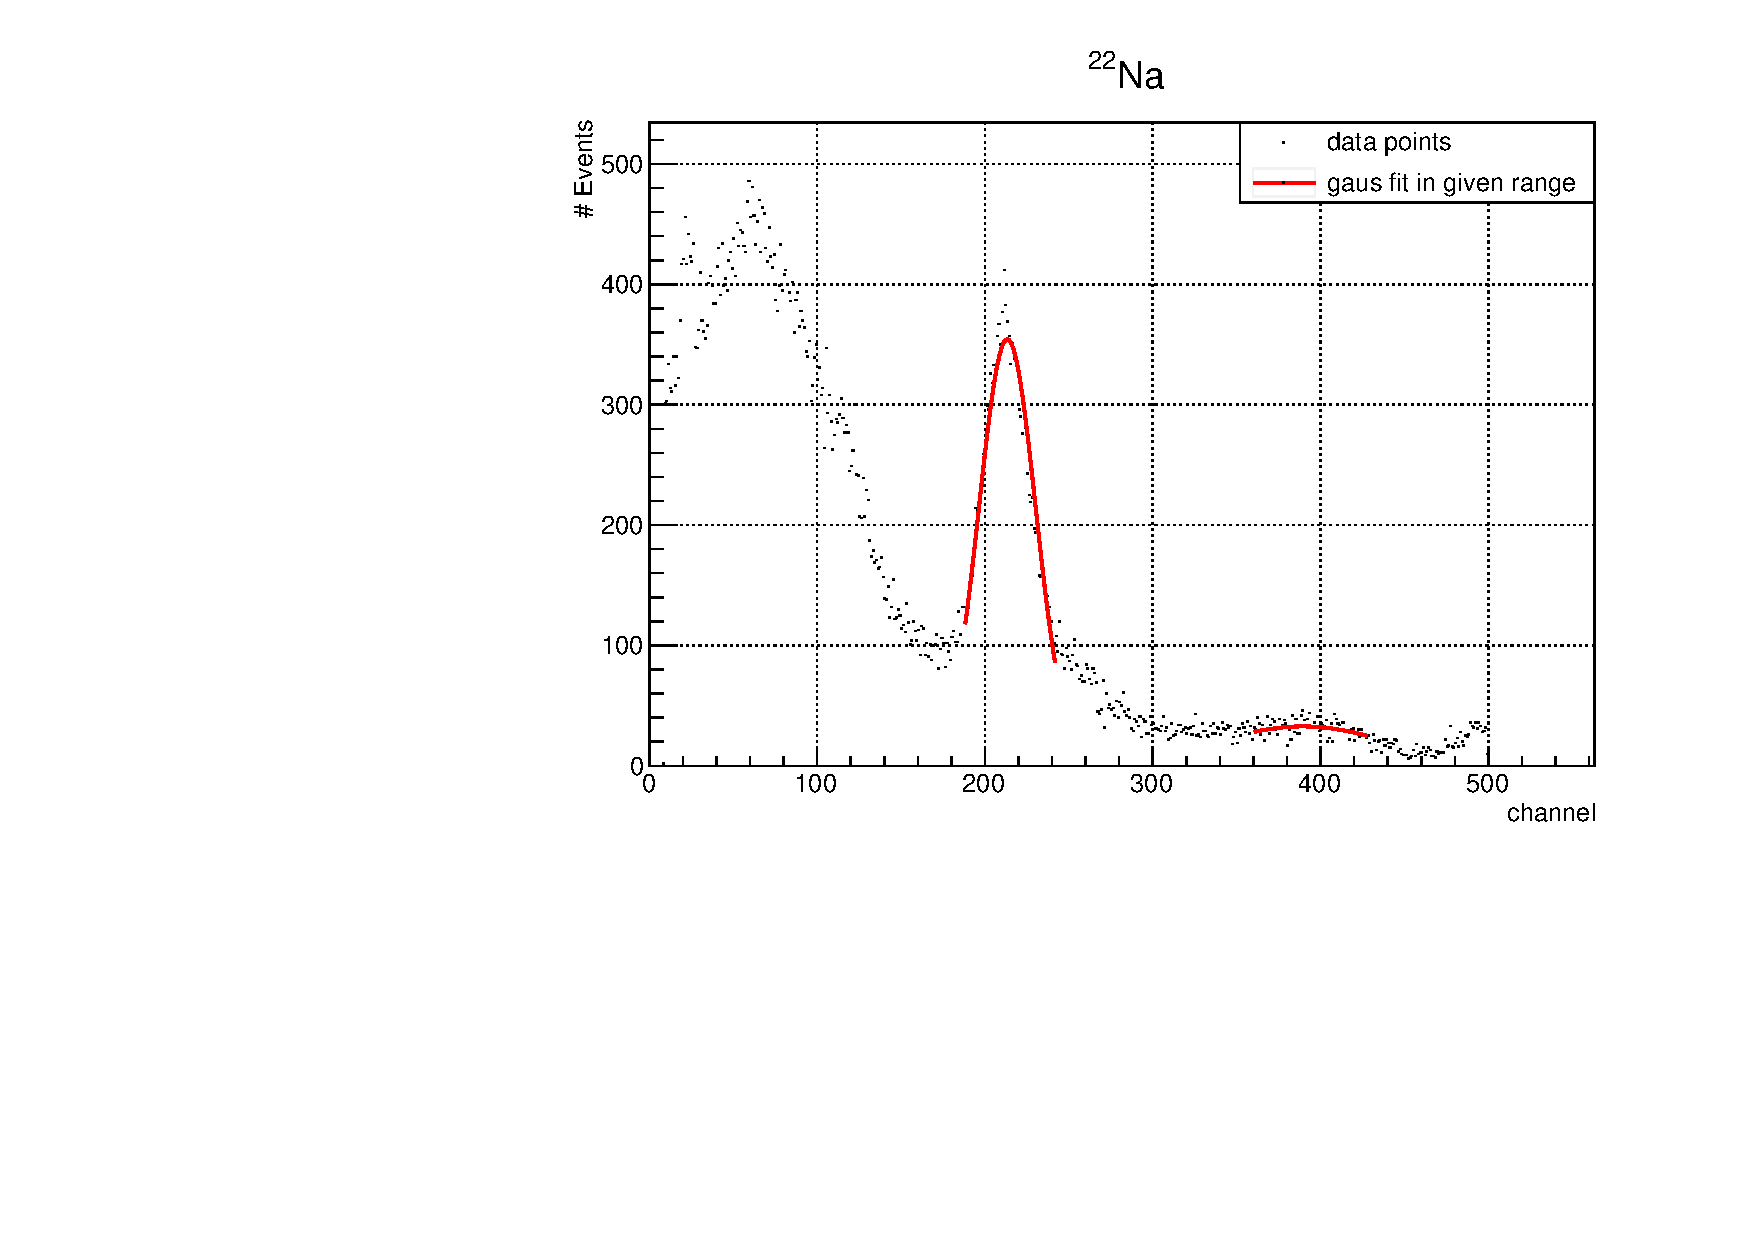
\includegraphics[scale=0.5]{./../plots/calibration/NA_22_fit.pdf}
\caption{Measured channels for ${}^{22}\mathrm{Na}$. At estimated ranges we fitted gaussian distributions to get better estimates of the peaks.}
\end{figure}

\newpage

\begin{figure}[h]
\centering
\caption{Measured channels and corresponding energies. Data for a linear fit.}
\vspace{0.2cm}
\begin{tabular}{lccc}
& mean & sigma & energy in keV \\
\hline
\hline
\vspace{0.1cm}
${}^{22}\mathrm{Na}$ & 213.33 & 16.88 & 511.0 \\
${}^{22}\mathrm{Na}$ & 389.31 & 52.35 & 1274.6 \\
$^{60}\mathrm{Co}$ & 362.87 & 68.07 & 1173.2 \\
$^{60}\mathrm{Co}$ & 463.79 & 32.98 & 1332.6 \\
$^{137}\mathrm{Cs}$ & 278.01 & 16.78 & 661.7 \\
\end{tabular}
\end{figure}

\begin{figure}[h]
\centering
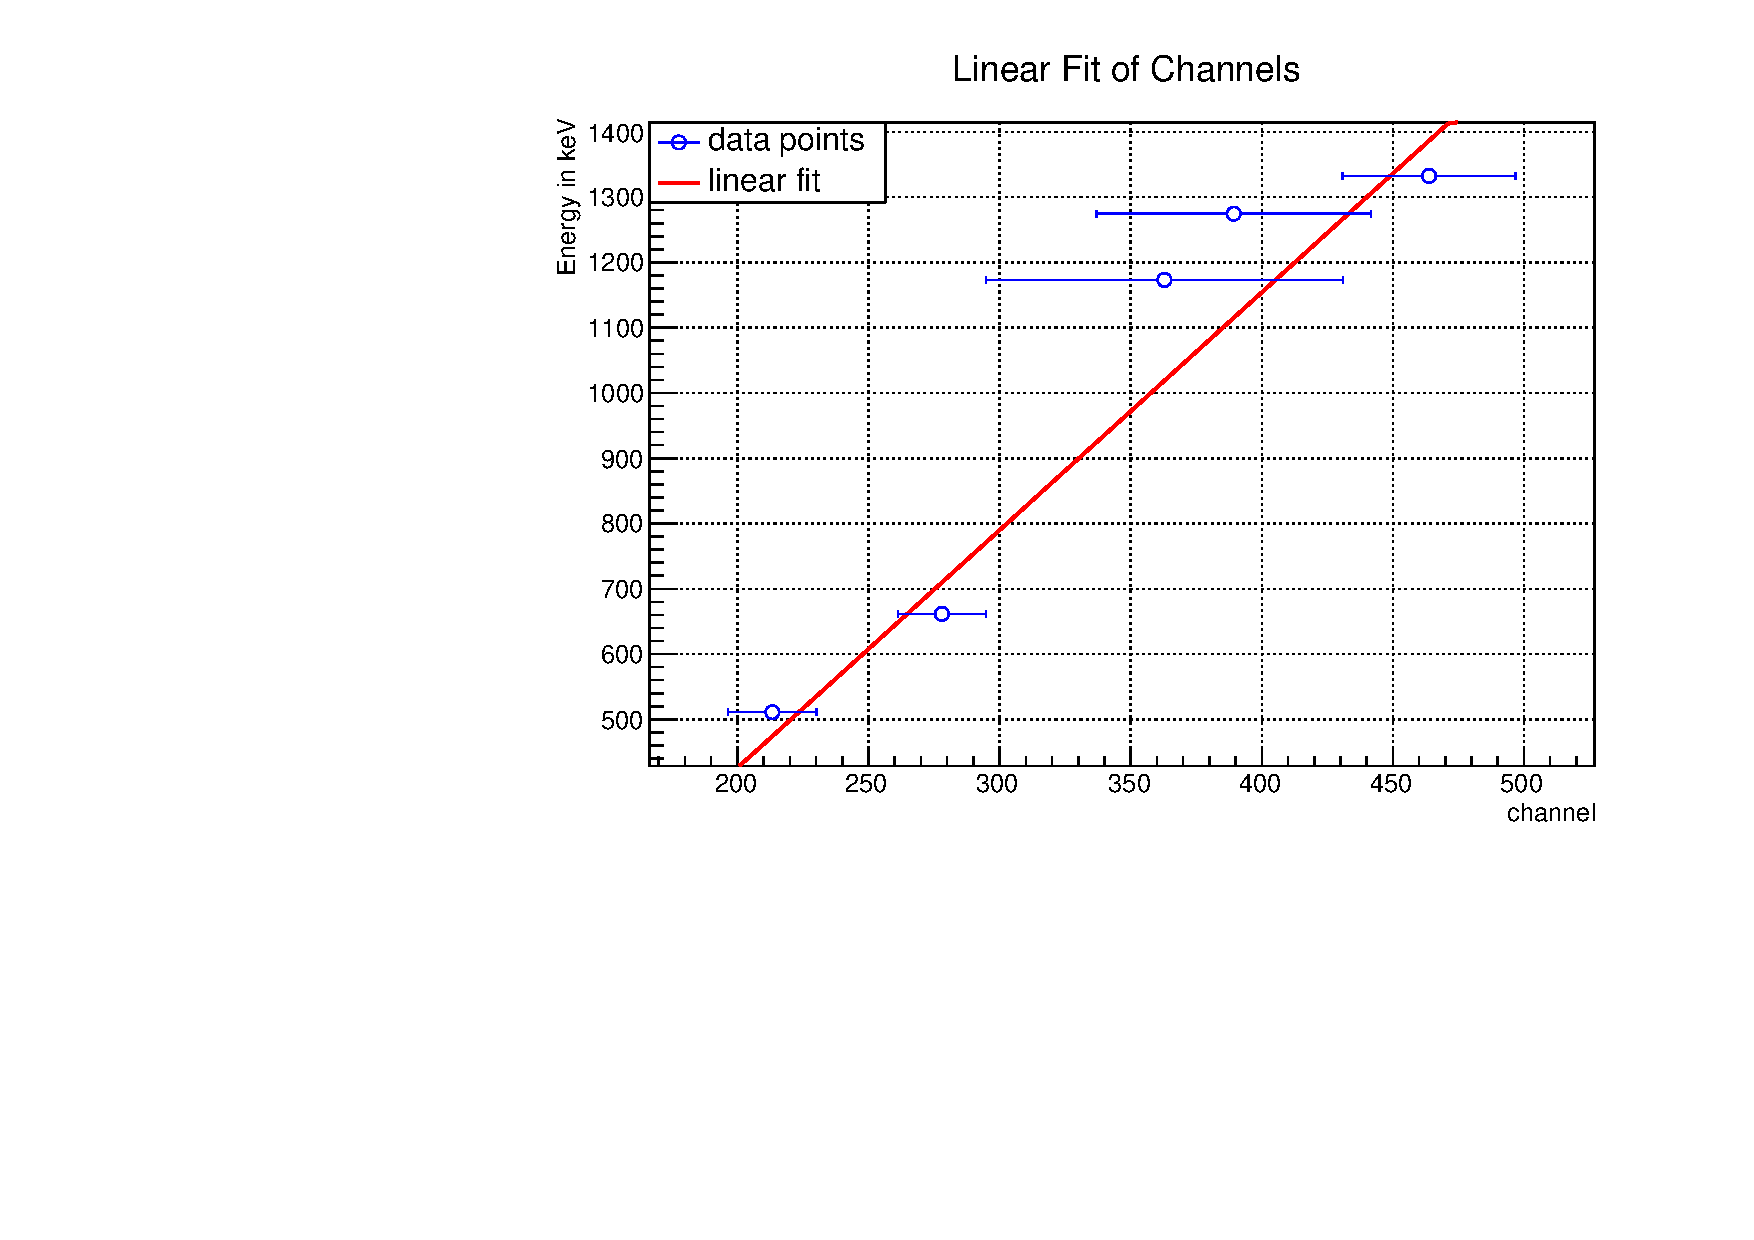
\includegraphics[scale=0.5]{./../plots/calibration/lin_fit.pdf}
\caption{Linear fit of channels and corresponding energies. The slope and intersection make it possible so that we can map the channels on the energies.}
\end{figure}


\newpage

\subsection{Differential Cross Section}

Next we measure the diffential cross section with respect to the solid angle $\Omega$. We assume that it has a rotation symmetry, i.e. it is independend of the azimuth $\phi$.\\
We change the angle in $10 ^{\circ}$ steps ranging from $20 ^{\circ}$ to $100 ^{\circ}$ and measure the background without target and the events with target. The sum of the difference is the total number scattered $R$. \\
To calculate the cross section we use the formular given in corresponding part of the preparation. 
$$\frac{d\sigma}{d\Omega} = \frac{R(\Delta \Omega)}{\Delta \Omega} \cdot \frac{1}{\Phi _0 n} \cdot \frac{1}{\epsilon} $$
To mention is the decay of the source, so we had to correct it by a factor $2^{-t/t_{1/2}}$ with $t_{1/2} = 30a$ and $t = 2016 - 1971 = 45a$. We also multiplied this value by the time we measured the events $t_{meassurement} = 300s$\\
The values used are the following:
$$ \Delta \Omega = \pi \cdot (d/2)^{2} / r^{2}_{target-crystal} = 1.10 \cdot 10^{-2}$$
$$n =  \frac{L}{A} \cdot Z \rho \pi (\frac{d}{2})^{2} \cdot l = 6.15 \cdot 10^{23}$$
$$\Phi_0 = (1.54 \pm 0.09) \cdot 10^{6} \mathrm{cm}^{-2} \mathrm{s}^{-1} $$
$$\frac{1}{\epsilon} = 2.08 \pm 0.01$$

Fig.2.5 shows the values of the polar angle $\Theta$, the measured cross section with its errors and the theoretical values from Klein-Nishina-Formular. These values are plotted in Fig.2.4. For bigger angles $\Theta$, the difference is bigger.\\

\newpage

\begin{figure}[h]
\centering
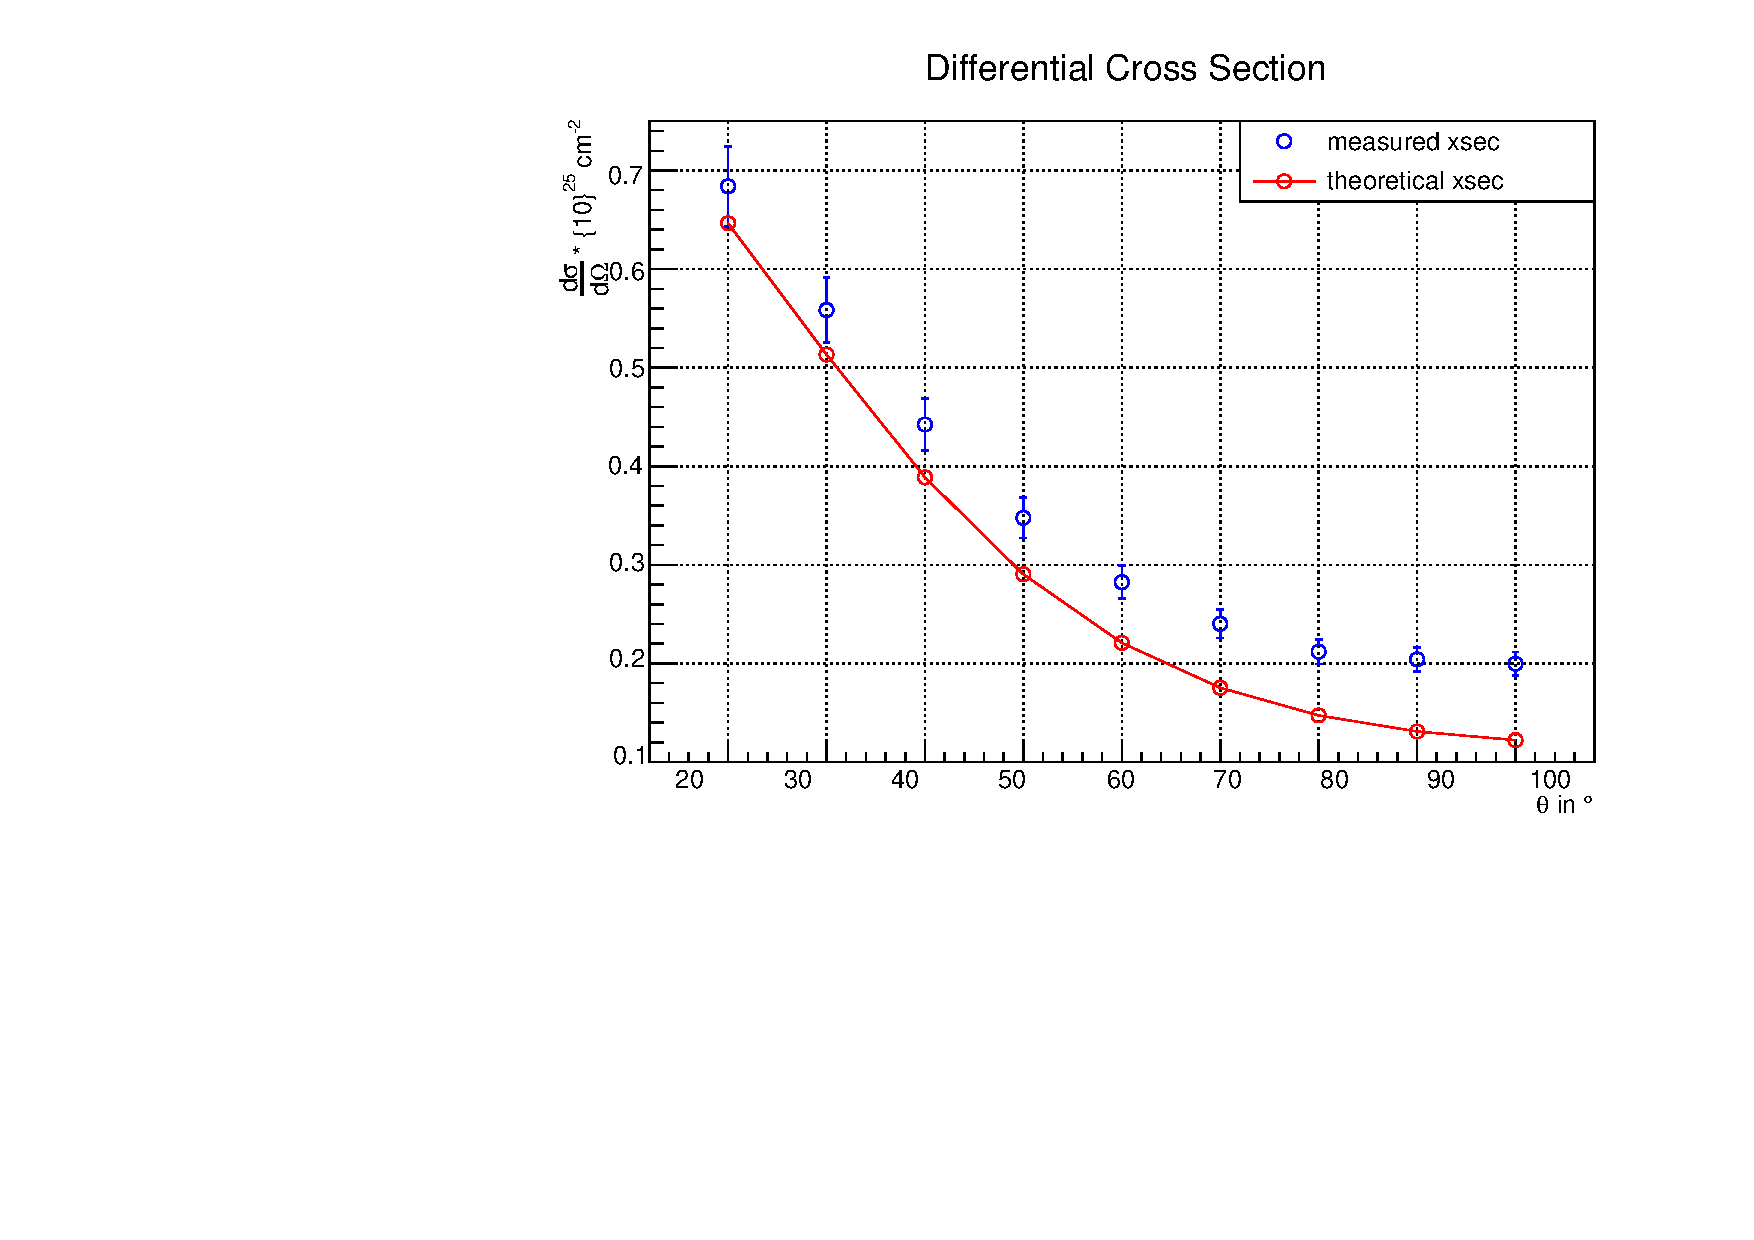
\includegraphics[scale=0.5]{./../plots/xs.pdf}
\caption{Measured and theoretical Cross section.}
\end{figure}

\begin{figure}[h]
\centering
\caption{Angles $\Theta$ and the measured differential cross section in $10^{25} \cdot cm^{2}$.}
\vspace{0.2cm}
\begin{tabular}{lccc}
$\Theta$ in ${}^{\circ}$ & $\frac{\mathrm{d}\sigma}{\mathrm{d}\Omega}$ in $10^{25} \cdot cm^{2}$ & error in $10^{25} \cdot cm^{2}$ & theoretical value in $10^{25} \cdot cm^{2}$ \\
\hline
\hline
%\vspace*{0.1cm}
20     &  0.684 & 0.041 & 0.646 \\
30     &  0.558 & 0.033 & 0.513 \\
40     &  0.442 & 0.026 & 0.389 \\
50     &  0.348 & 0.021 & 0.290 \\
60     &  0.282 & 0.017 & 0.221 \\
70     &  0.240 & 0.014 & 0.175 \\
80     &  0.212 & 0.013 & 0.147 \\
90     &  0.204 & 0.012 & 0.131 \\
100    &  0.200 & 0.012 & 0.122 \\
\end{tabular}
\end{figure}

\newpage

\subsection{Energy Shift and Invariant Mass of Electrons}

The energy of a fixed angle is determined by a gaussian fit, an example is shown in Fig.2.6 for $\Theta = 50^{\circ}$. The procedure is the same as in the calibration subsection above. Using the measured linear fit from above we can acquire the energies given the channels.\\
Using the results calculated in the calibration and using the deviation of the gaus distributions for the channel error we find the energy:
$$E = (-302.81 + 3.64 \cdot \mathrm{channel}) \ keV $$
$$\sigma_E^{2} = (148.21^{2} + \mathrm{channel}^{2} \cdot 0.51^{2} + 3.64^{2} \cdot \sigma_{channel}^{2}) \ keV $$
In the equation for the error you can see that there is a part, $(148.21 \ keV)^{2}$, which does not depend on the channel or the deviation of it. This originates from the y-intersect of the calibration fit. For small channel numbers and small errors of the channel number, this becomes the dominating part. The result is a big relative uncertainty for big values of the inverse energy $\frac{1}{E}$, which is the reason for the appereance of the graph below.
The fit results and the corresponding energies for each angle $\Theta$ are given in Fig.2.7.

\vspace*{1.5cm}

\begin{figure}[h]
\centering
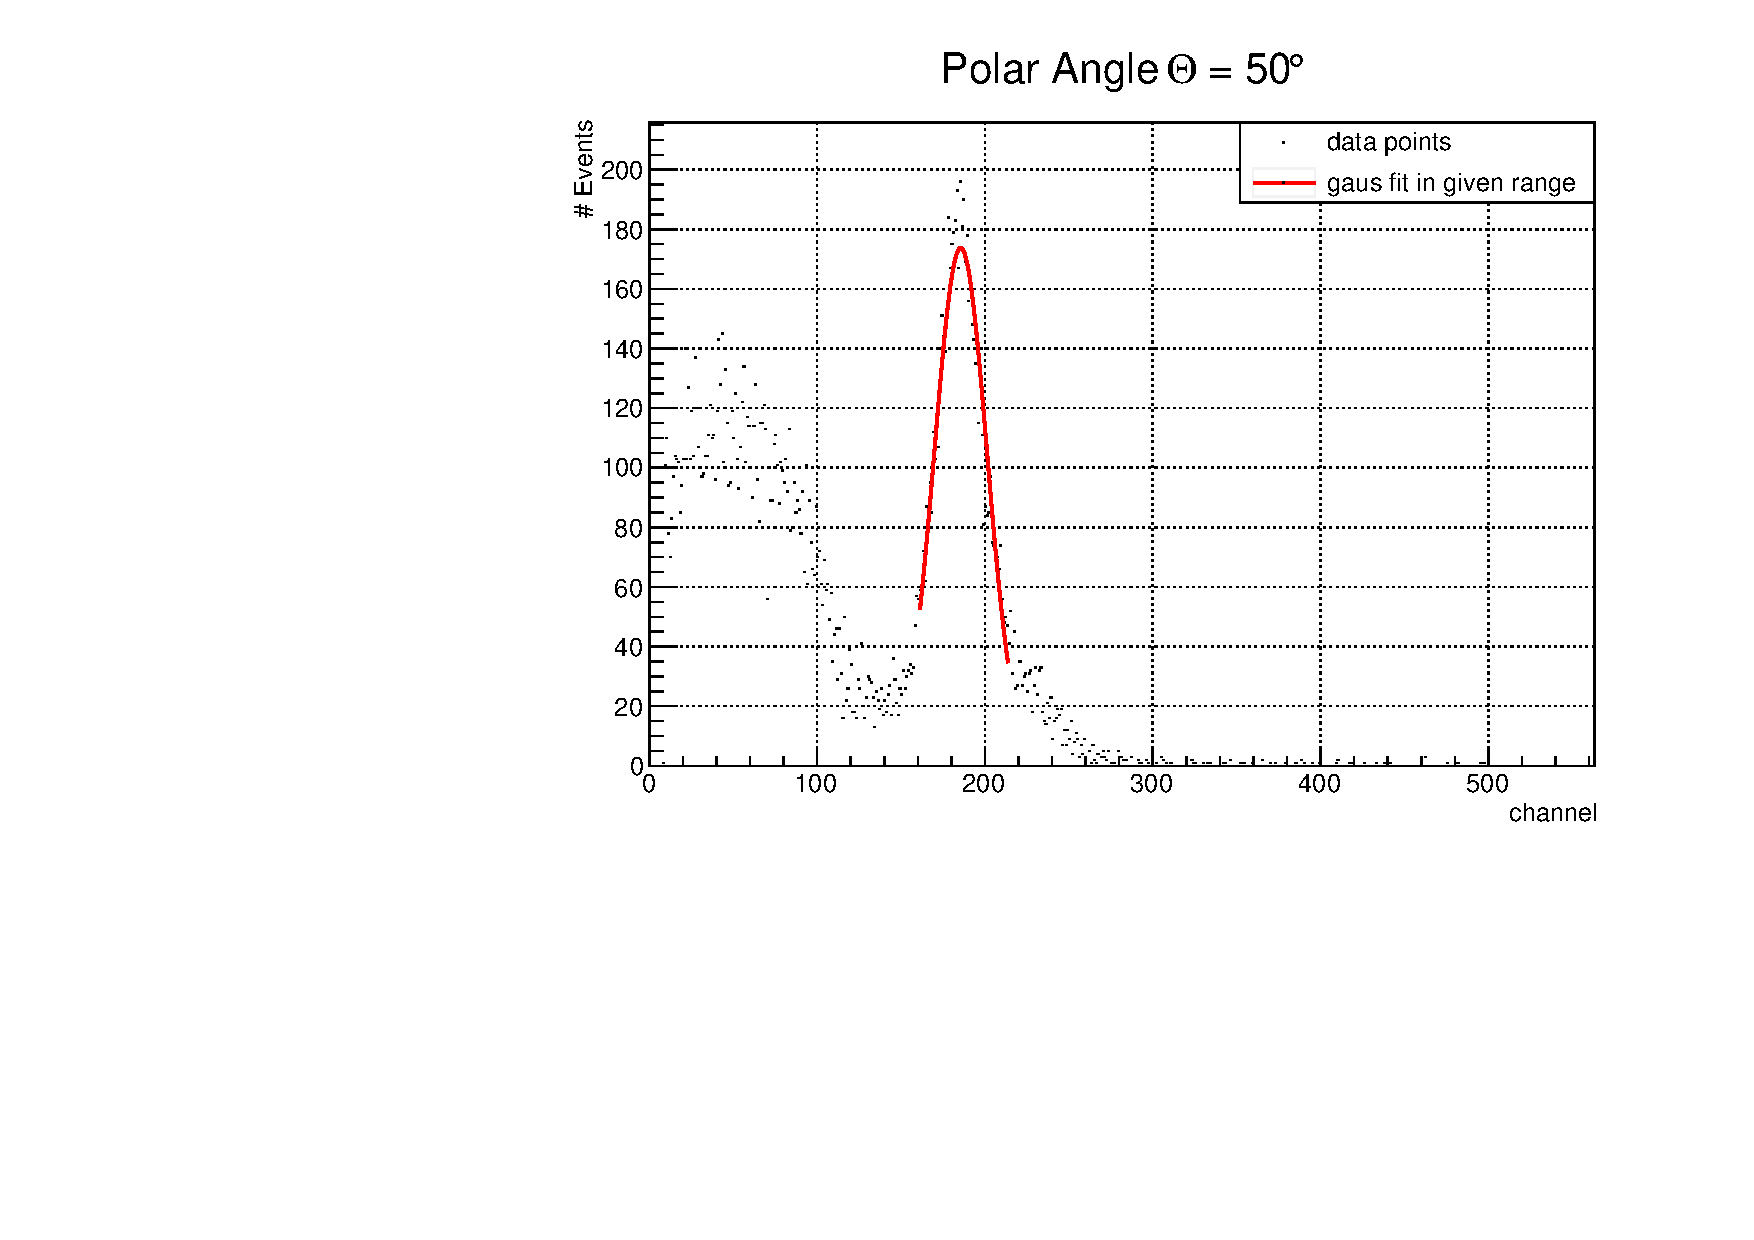
\includegraphics[scale=0.5]{./../plots/50_deg.pdf}
\caption{Fit to determine the energy at a fixed angle of $\Theta = 50^{\circ}$.}
\end{figure}

\newpage


\begin{figure}[h]
\centering
\caption{Channels with errors given by gaussian fits and corresponding energies with errors for each angle $\Theta$}
\vspace{0.2cm}
\begin{tabular}{lcccc}
Angle $\Theta$ in ${}^{\circ}$ & Channel & Deviation & Energy in $keV$ & $\sigma _ {Energy}$ in $keV$ \\
\hline
\hline
%\vspace*{0.1cm}
20 & 92.79     &  9.28 & 35.18 & 159.30 \\
30 &104.78     &  11.40 & 78.83 & 163.04 \\
40 &119.50     &  12.34 & 132.45 & 166.58 \\
50 &138.39     &  14.43 & 201.24 & 172.56 \\
60 &160.93     &  16.72 & 283.35 & 180.28 \\
70 &185.53     &  15.68 & 372.96 & 185.20 \\
80 &211.99     &  17.88 & 469.33 & 195.06 \\
90 &237.73     &  19.34 & 563.07 & 204.51 \\
100 &261.00    &  20.08 & 647.80 & 212.75 \\
\end{tabular}
\end{figure}


As described in the preparation we have the equation
$$\frac{1}{E'} = \frac{1}{E} + \frac{1}{m_0 \cdot c^{2}} \cdot (1 - \cos \Theta) $$
So we plot the inverse energy $\frac{1}{E}$ over $1 - \cos(\Theta)$. The inverse of the slope gives then the invariant mass of the electron in $keV$. The resulting parameters are given by:
$$\mathrm{y-intercept} = (1.20237 \pm 0.553517) \cdot 10^{-4} \ keV^{-1}$$
$$\mathrm{slope} =  (4.55878 \pm 3.02294) \cdot 10^{-3} \ keV^{-1}$$
As a result we can calculate the electron mass to be:
$$(219.357 \pm 145.456) \ keV$$

The results are not good which can be seen by comparing them with the values it should be, namely $m_e \approx 515 \ keV$ and $(\mathrm{y-intercept})^{-1} = E_{Cs_137} \approx 602 \ keV$. The problem here is the big relative deviation of the inverse energies. To get better results we keep the y-intersect constant at the known $1/(602 \ keV)$. The resulting plot is given in Fig.2.8, which looks in this scaling really similiar to the plot with variable intersect. The resulting parameter is:
$$slope = (2.59972 \pm 1.88442) \cdot 10^{-3} \ keV^{-1}$$
The final result for the electron mass is therefore:
$$m_e = (384.66 \pm  278.82) \ keV$$
The theoretical value of $m_e = 602 \ keV$ lies withing one standard deviation of our result.



\newpage

\begin{figure}
\centering
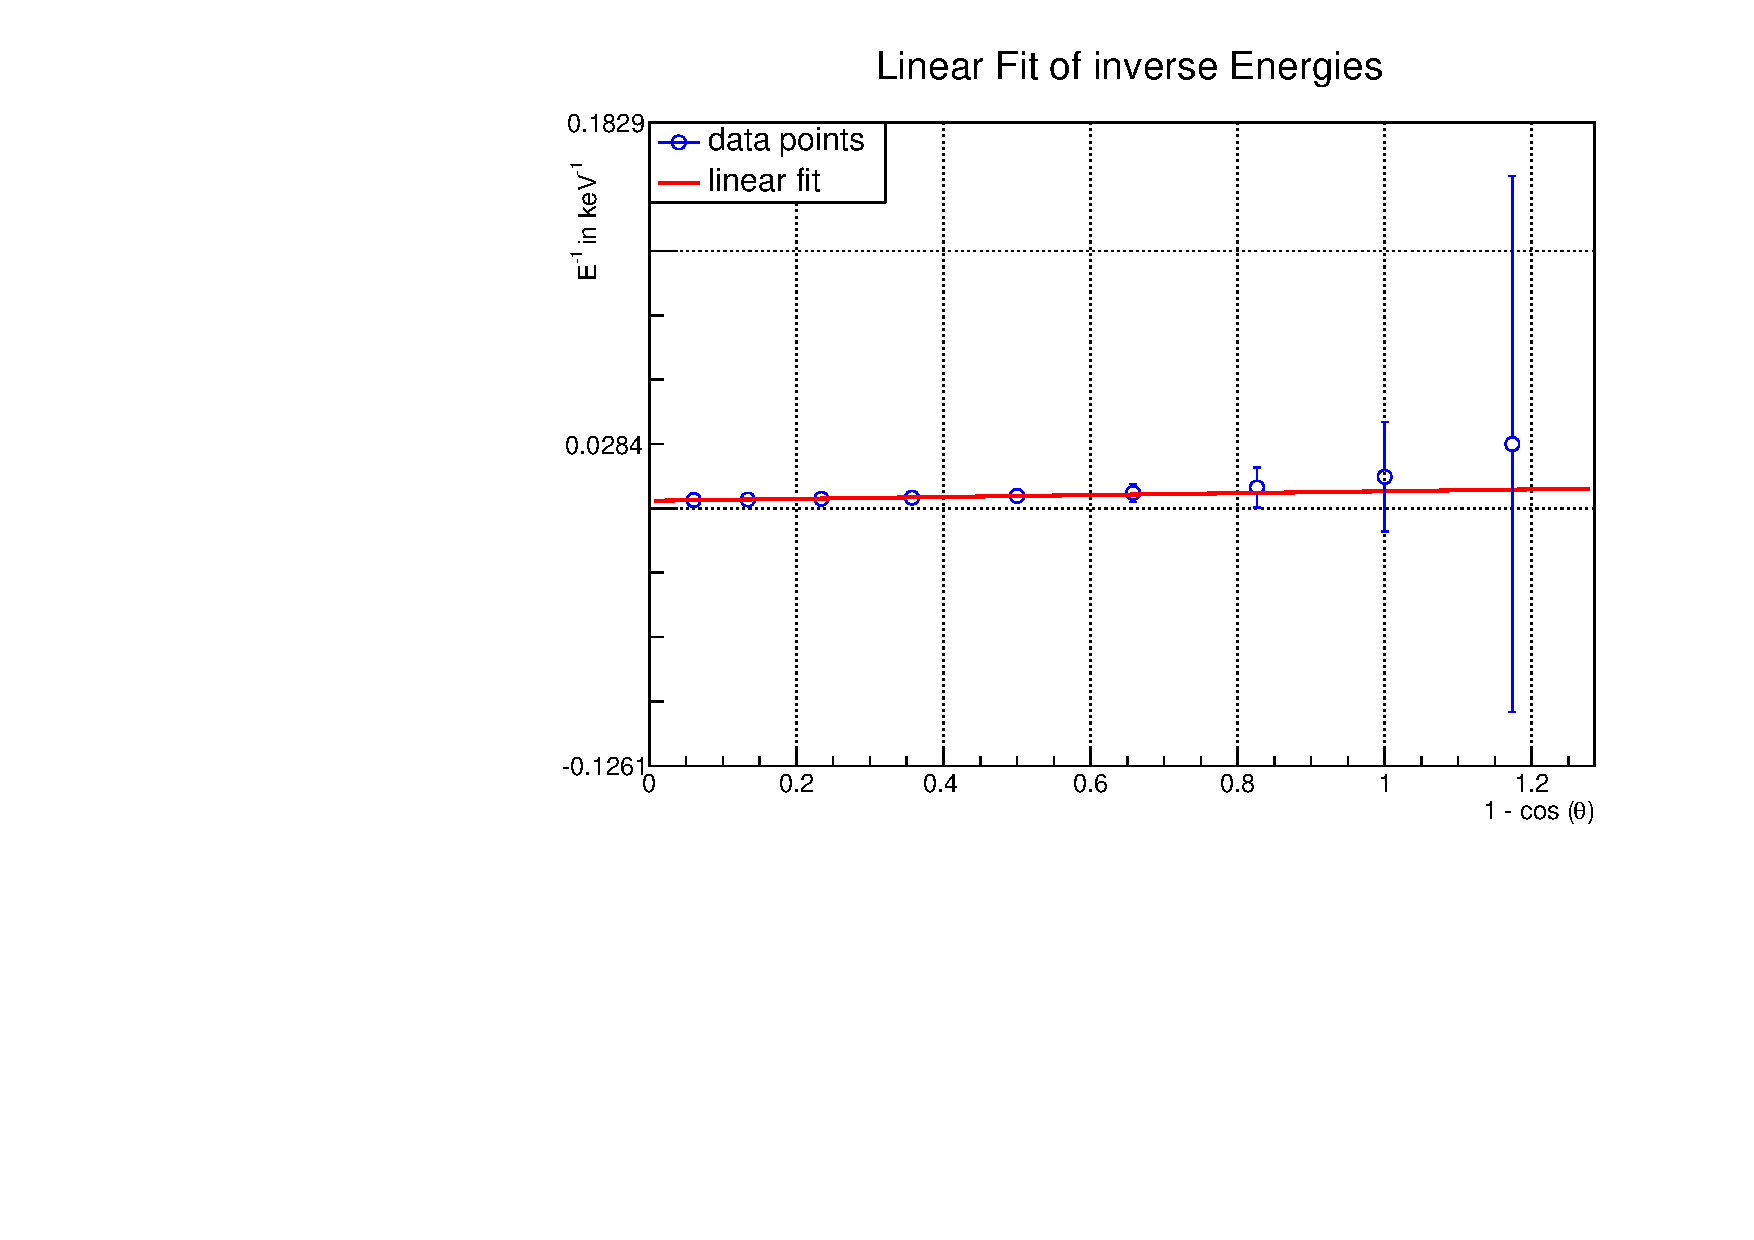
\includegraphics[scale=0.5]{./../plots/inv_el_mass.pdf}
\caption{Fit to determine the invariant mass of electrons. The uncertainty is big for high values of $\frac{1}{E}$ due to the big uncertainty of the y-intercept in the calibration fit.}
\end{figure}


\subsection{Cross Section for Different Materials}

As described in the preparation the following formular should be true given that the binding energy is much smaller than the energy of the photons:
$$(\frac{\mathrm{d}\sigma}{\mathrm{d}\Omega})_e = const. \cdot R \frac{A}{\rho Z} $$
We measured the total number of events for a fixed angle $\Theta = 20 ^{\circ}$ for different targets and subtracted the background $R = R_{target} - R_{background}$. The materials are aluminium, copper, iron and lead. Each target has the same size and shape. \\
To check the formular above we plot $\frac{R \cdot A}{\rho Z}$ over $Z$. This should be a horizontal line. Here $A$ is the atomic mass, $\rho$ is the density of the material and $Z$ is the atomic number. The used values are given in Fig.2.9.\\
\\
The resulting graph is shown in Fig.2.10. All data points except the one for lead are on a horizontal line. The reason is that the binding energy of lead is higher than for the others. Therefore the equation above doesn't hold true anymore because the electrons can't be simplified to be free anymore. It seems that with increasing atomic number, the error gets bigger. 

\newpage

\begin{figure}[h]
\centering
\caption{Values used for the different materials in the equation above.}
\vspace{0.2cm}
\begin{tabular}{lcccc}
 & aluminium  & copper & iron & lead  \\
\hline
\hline
$\rho$ in $\frac{g}{cm^{3}}$ & 2.70 & 8.92 & 7.87 & 11.34 \\
$A$ in $u$ & 26.98 & 63.55 & 55.85 & 207.2 \\
$Z$ & 13 & 29 & 26 & 82 \\
$R$ & 19619 & 58964 & 55038 & 50573 \\
$\sigma (R)$ & 1265.54 & 3688.28 & 3455.20 & 3477.25 \\
\end{tabular}
\end{figure}


\begin{figure}[h]
\centering
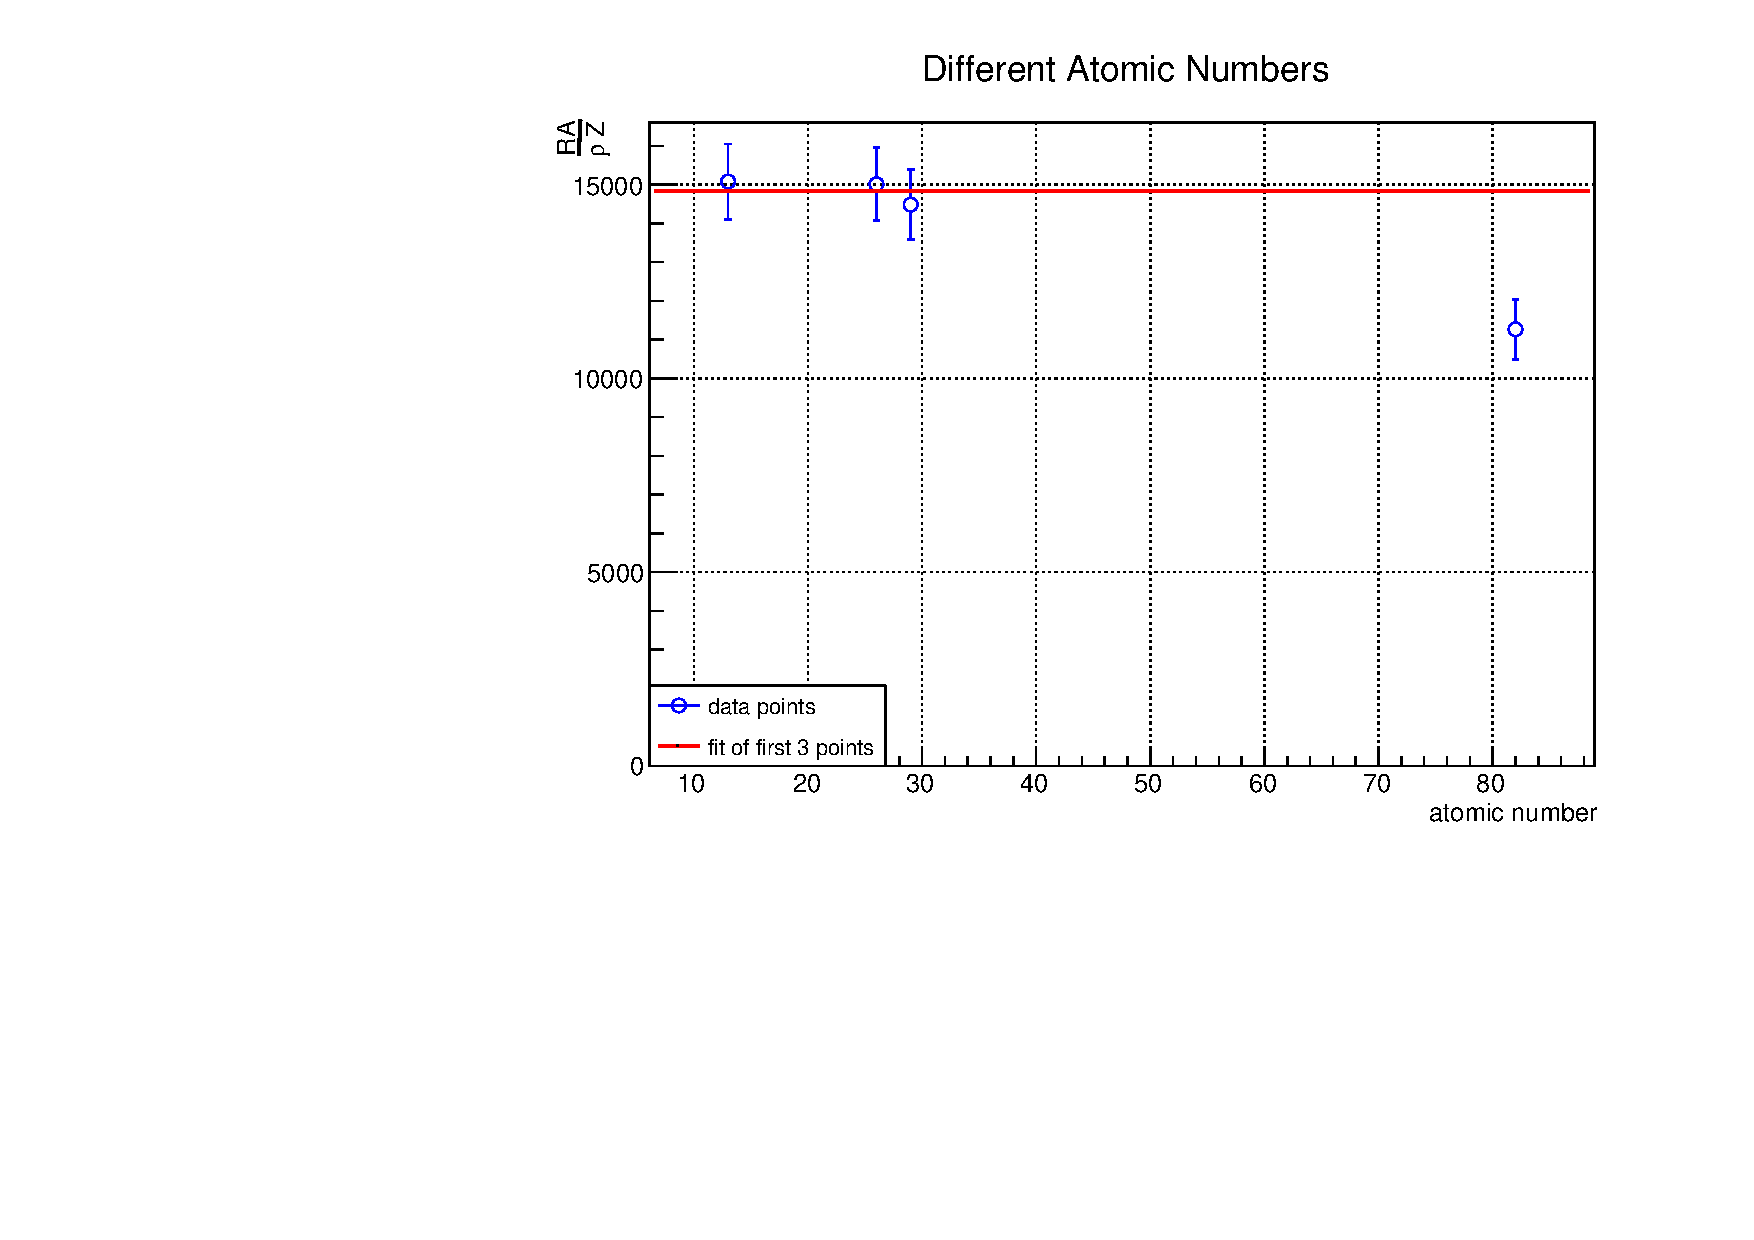
\includegraphics[scale=0.5]{./../plots/part_c.pdf}
\caption{Plot of the quantity mentioned in the text over the atomic number Z with a fit of the first three data points. Lead doesn't align with the other materials. The reason is the binding energy of the electrons.}
\end{figure}

\newpage

\subsection{Conclusion}

We calibrated the systems by calculating the corresponding energies for each channel. This was done by a linear fit. Our result cannot be compared with theoretical values, since it depends strongly on the experimental setup. \\
Next the differential cross section was calculated with respect to the solid angle $\Omega$. Our results differ from the theoretical values given by the Klein-Nishina-Formular. The difference is bigger for larger angles. This seems to be a systematic uncertainty given by the experimental setup. \\
In the third paragraph the invariant mass of electrons was measured using the energy shift of the compton scattering. Here we had to use the theoretical value of the photons emitted by ${}^{137}Cs$ to get a reasonable result. Using this we found a good result. The theoretical value lies within one standard deviation of our calculated value. \\
Lastly we compared the cross section of different materials. For aluminium, copper and iron the results align reasonably well with our prediction. For lead the binding energy is too high and therefore the requirements are not fulfilled.
